\chapter{%
実験}

RGB-Dカメラから取得したデータセットをRXDネットワークを使用し曲管又はT字管を認識できるか検証する。
物体認識においては他のネットワークでも実験し、RXDネットワークの有用性を確かめる。

\section{評価指標}
物体認識の評価指標ではパラメータ数(Params), Intersection over Union(IoU), mean Average Precision(mAP)を用い認識ネットワークの性能評価を行う。
まず、パラメータ数は認識ネットワークの学習可能なパラメータの合計数を示す。これにより、認識ネットワークの複雑度を示すことができる。
次に。IoUは正解と予測のバウンディングボックスの共通の重なり部分を2つのバウンディングボックスを重ねたときの総面積で除算したものである。
IoUは0~1.0の値の範囲で示され、値が大きければ大きいほどラベル付されたボックスと予測されたボックスの重なりが正しいことになり、正確に認識していると判断できる。
次に、mAPは1つ1つのクラスに対して平均適合率であるAP(Average Precision)を計算する。まず、モデルの予測結果を、出力する信頼度スコア順に並べる。
ラベルごとに信頼度スコアがそのラベルの値以上の予測結果について、適合率と再現率を求める。適合率と再現率は図4.1のようにTrue Positive(TP)とFalse Negative(FN)を用いて表される。
その適合率と再現率のグラフから適合率の下側の面積を求める。ここで、予測されたラベルが正解なのかの判断はIoUが決められたしきい値以上で、最も信頼度スコアが高い予測ラベルが正解とするように判断される。
そして最後に、クラスごとに計算されたAPの平均を算出したものがmAPになる。

\begin{figure}[htbt]
	\centering
	 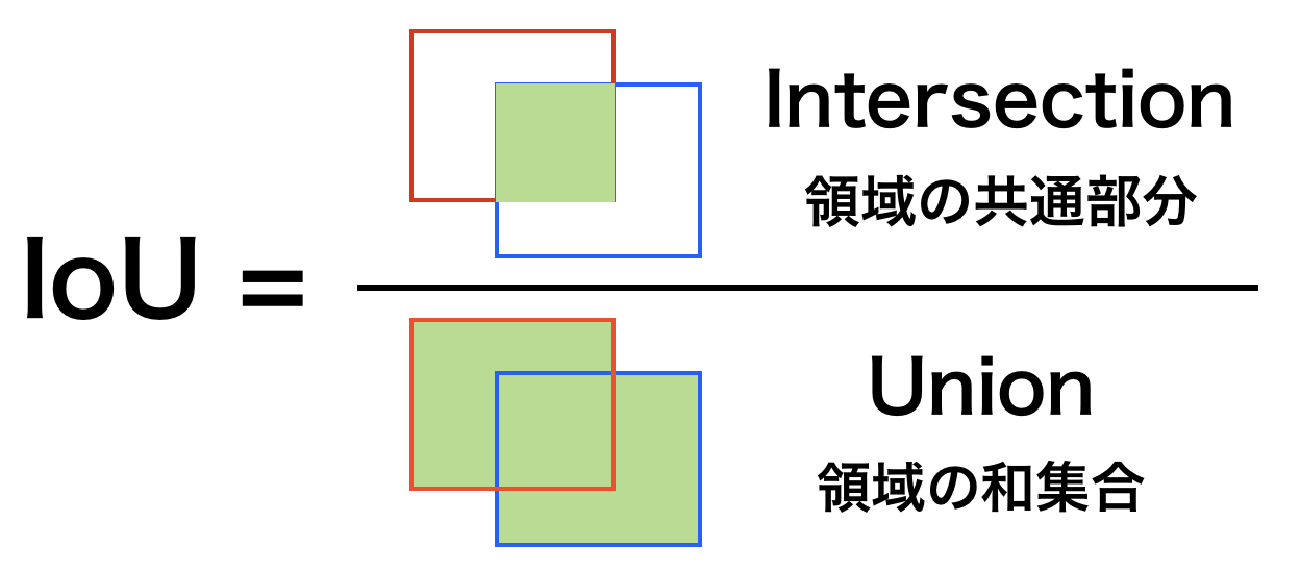
\includegraphics[height=45mm]{iou.eps}
	 \caption{Intersection over Union(IOU)}
	 \label{fig:f2}
\end{figure}

\begin{figure}[htbt]
	\centering
	 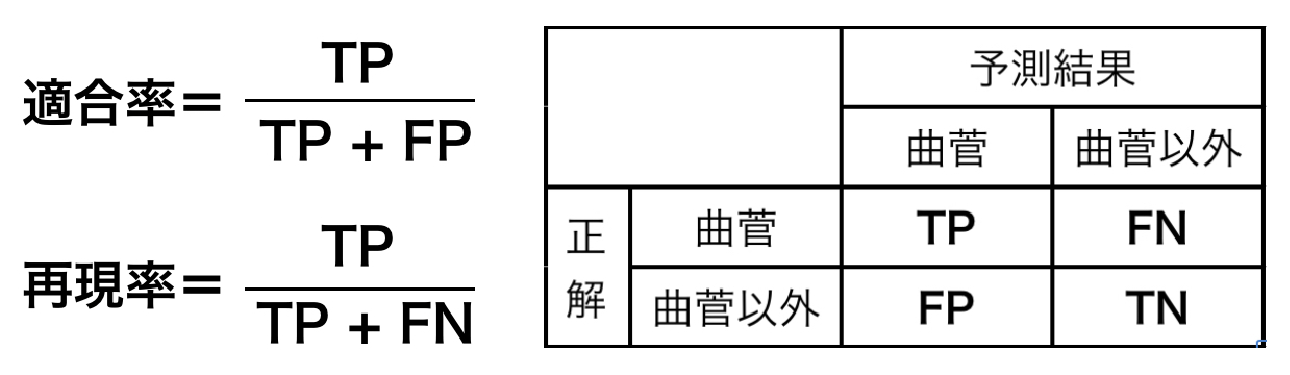
\includegraphics[height=35mm]{recall.eps}
	 \caption{適合率と再現率}
	 \label{fig:f2}
\end{figure}


\section{結果と考察}
\subsection{物体検出}

